\documentclass[12pt]{article}
\usepackage[margin=2.5cm]{geometry}
\usepackage{enumerate}
\usepackage{amsfonts}
\usepackage{amsmath}
\usepackage{fancyhdr}
\usepackage{amsmath}
\usepackage{amssymb}
\usepackage{amsthm}
\usepackage{mdframed}
\usepackage{graphicx}
\usepackage{subcaption}
\usepackage{adjustbox}
\usepackage{listings}
\usepackage{xcolor}
\usepackage{booktabs}
\usepackage[utf]{kotex}

\definecolor{codegreen}{rgb}{0,0.6,0}
\definecolor{codegray}{rgb}{0.5,0.5,0.5}
\definecolor{codepurple}{rgb}{0.58,0,0.82}
\definecolor{backcolour}{rgb}{0.95,0.95,0.92}

\lstdefinestyle{mystyle}{
    backgroundcolor=\color{backcolour},
    commentstyle=\color{codegreen},
    keywordstyle=\color{magenta},
    numberstyle=\tiny\color{codegray},
    stringstyle=\color{codepurple},
    basicstyle=\ttfamily\footnotesize,
    breakatwhitespace=false,
    breaklines=true,
    captionpos=b,
    keepspaces=true,
    numbers=left,
    numbersep=5pt,
    showspaces=false,
    showstringspaces=false,
    showtabs=false,
    tabsize=1
}

\lstset{style=mystyle}

\begin{document}
\title{CSC236 Worksheet 2 Solution}
\author{Hyungmo Gu}
\maketitle

\section*{Question 1}
\begin{itemize}
    \item

    \bigskip

    \underline{\textbf{Statement:}} Any full binary tree with at least 1 node has
    more leaves than internal nodes.

    \bigskip

    \begin{proof}
    Let $n$ be the total number of nodes in a full binary tree.

    \bigskip

    We will prove the statement by complete induction on $n$.

    \bigskip

    \underline{\textbf{Base Case ($n = 1$):}}

    \bigskip

    Let $n = 1$.

    \bigskip

    We need to prove the full binary tree with 1 total number of nodes
    has more leaves than internal nodes.

    \bigskip

    There is only one full binary tree exists with 1 total number of node. That is,
    the full binary tree with 1 child node and 0 internal nodes.

    \bigskip

    Then, since we know a node is a leaf if it has no children, and since we know
    the child node has 0 children, we can write the child node is a leaf node.

    \bigskip

    Then, because we know the full binary tree has 1 leaf node, and 0 internal node,
    we can conclude it has more leaves than internal nodes.

    \bigskip

    \underline{\textbf{Base Case ($n = 2$):}}

    \bigskip

    Let $n = 2$.

    \bigskip

    We need to prove the full binary tree with 2 total number of nodes
    has more leaves than internal nodes.

    \bigskip

    The definition of full binary tree tells us that a binary tree is a full
    binary tree if every internal node has two children.

    \bigskip

    Since we know the tree with 2 total number of nodes
    has 1 leaf and 1 internal node, using above fact, we can write the
    tree is not a full binary tree.

    \bigskip

    Then, by vacuous truth, we can conclude the tree has more leaves than
    internal nodes.

    \bigskip

    \underline{\textbf{Base Case ($n = 3$):}}

    \bigskip

    Let $n = 3$.

    \bigskip

    We need to prove the full binary tree with 3 total number of nodes
    has more leaves than internal nodes.

    \bigskip

    The definition of full binary tree tells us that a binary tree is a full
    binary tree if every internal node has two children.

    \bigskip

    Because we know there are two types of binary trees possible,
    one is the tree with 2 internal nodes and 1 child and the other
    is 1 internal node and 2 children, using above fact, we can write
    the only possible full binary tree with 3 total nodes is 1 internal
    node and 2 children.

    \bigskip

    Now, the definition of leaf tells us leaf is a node that has no children.

    \bigskip

    Because we know by observation that the 2 child nodes don't
    have children, we can write the full binary tree has 2 leaves.

    \bigskip

    So, because we know the full binary tree has 1 internal node
    and 2 leaves, we can conclude the full binary tree has more
    leaves than internal node.

    \bigskip

    \underline{\textbf{Inductive Step:}}

    \bigskip

    Let $k \geq 1$ be an arbitrary natural number. Assume that for all natural
    number $i$ satisfying $1 \leq i \leq k$, any full binary trees with $i$
    total number of nodes has more leaves than internal nodes.

    \bigskip

    Let $T$ be an arbitrary full binary tree with $k+1$ nodes. Let $T'$
    be the binary tree obtained by removing 2 leaves from the same parent
    node.


    \bigskip

    Let $\ell$ be the number of leaves of $T$, and $m$ be the number of
    internal nodes of $T$. Similarly, let $\ell'$ be the number of leaves of
    $T'$ and $m'$ be the number of internal nodes of $T'$. We must prove
    $l > m$.

    \bigskip

    First, we need to show $\ell' > m'$.

    \bigskip

    The header tells us that $T'$ is a full binary tree as a result
    of removing 2 leaves from the parent node of $T$.

    \bigskip

    Using this fact, we can calculate $T'$ has
    \setcounter{equation}{0}
    \begin{align}
        k+1-2 = k-1
    \end{align}

    nodes.

    \bigskip

    Then, because we know $1 \leq k-1 \leq k$, using induction hypothesis,
    we can write

    \begin{align}
        \ell' > m'
    \end{align}

    \bigskip

    Second, we need to show $\ell = \ell' + 1$ and $m = m' + 1$.

    \bigskip

    The total number of both the leaf nodes and the internal
    nodes increase by 1 when 2 nodes are added to the same leaf node
    in a full binary tree.

    \bigskip

    Since 2 nodes added to the same leaf node of $T'$ is $T$, we can
    write $\ell = \ell' + 1$ and $m = m' + 1$.

    \bigskip

    Finally, putting together, because we know $\ell' > m'$, $\ell = \ell' + 1$
    and $m = m' + 1$, we can conclude

    \begin{align}
        \ell' + 1 &> m' + 1\\
        \ell &> m
    \end{align}


    \end{proof}

    % \begin{mdframed}
    %     \underline{\textbf{Rough Work:}}

    %     \bigskip

    %     Let $n$ be the total number of nodes in a full binary tree.

    %     \bigskip

    %     We will prove the statement by complete induction on $n$.

    %     \bigskip

    %     \begin{enumerate}[1.]
    %         \item Base Case ($n = 1$)

    %         \bigskip

    %         Let $n = 1$.

    %         \bigskip

    %         We need to prove the full binary tree with 1 total number of nodes
    %         has more leaves than internal nodes.

    %         \bigskip

    %         \begin{itemize}
    %             \item Show only one full binary tree exists with 1 total number of nodes.

    %             \begin{mdframed}
    %             There is only one full binary tree exists with 1 total number of node. That is,
    %             the full binary tree with 1 child node and 0 internal nodes.

    %             \end{mdframed}

    %             \item Show the child node is a leaf

    %             \begin{mdframed}
    %             Then, since we know a node is a leaf if it has no children, and since we know
    %             the child node has 0 children, we can write the child node is a leaf node.
    %             \end{mdframed}

    %             \item Conclude the full binary tree has more leaves than internal nodes
    %             \begin{mdframed}
    %             Then, because we know the full binary tree has 1 leaf node, and 0 internal node,
    %             we can conclude it has more leaves than internal nodes.
    %             \end{mdframed}
    %         \end{itemize}

    %         \begin{mdframed}

    %         \underline{\textbf{Base Case ($n = 1$):}}

    %         \bigskip

    %         Let $n = 1$.

    %         \bigskip

    %         We need to prove the full binary tree with 1 total number of nodes
    %         has more leaves than internal nodes.

    %         \bigskip

    %         There is only one full binary tree exists with 1 total number of node. That is,
    %         the full binary tree with 1 child node and 0 internal nodes.

    %         \bigskip

    %         Then, since we know a node is a leaf if it has no children, and since we know
    %         the child node has 0 children, we can write the child node is a leaf node.

    %         \bigskip

    %         Then, because we know the full binary tree has 1 leaf node, and 0 internal node,
    %         we can conclude it has more leaves than internal nodes.

    %         \end{mdframed}

    %         \item Base Case ($n = 2$)

    %         \begin{mdframed}

    %         \underline{\textbf{Base Case ($n = 2$):}}

    %         \bigskip

    %         Let $n = 2$.

    %         \bigskip

    %         We need to prove the full binary tree with 2 total number of nodes
    %         has more leaves than internal nodes.

    %         \bigskip

    %         The definition of full binary tree tells us that a binary tree is a full
    %         binary tree if every internal node has two children.

    %         \bigskip

    %         Since we know the tree with 2 total number of nodes
    %         has 1 leaf and 1 internal node, using above fact, we can write the
    %         tree is not a full binary tree.

    %         \bigskip

    %         Then, by vacuous truth, we can conclude the tree has more leaves than
    %         internal nodes.
    %         \end{mdframed}

    %         \item Base Case ($n = 3$)

    %         Let $n = 3$.

    %         \bigskip

    %         We need to prove the full binary tree with 3 total number of nodes
    %         has more leaves than internal nodes.

    %         \begin{enumerate}[1.]
    %             \item Show the three forms a full binary tree
    %             \begin{itemize}
    %                 \item State the definition of full binary tree

    %                 \begin{mdframed}
    %                 The definition of full binary tree tells us that a binary tree is a full
    %                 binary tree if every internal node has two children.
    %                 \end{mdframed}

    %                 \item Show that with 3 as the total number of nodes, the only full binary
    %                 tree that can be formed is 1 internal node and 2 children.

    %                 \begin{mdframed}
    %                 Because we know there are two types of binary trees possible,
    %                 one is the tree with 2 internal nodes and 1 child and the other
    %                 is 1 internal node and 2 children, using above fact, we can write
    %                 the only possible full binary tree with 3 total nodes is 1 internal
    %                 node and 2 children.
    %                 \end{mdframed}

    %                 \item Conclude that the children are leaves, and there are more
    %                 leaves than internal nodes

    %                 \begin{mdframed}
    %                 Now, the definition of leaf tells us leaf is a node that has no children.

    %                 \bigskip

    %                 Because we know by observation that the 2 child nodes don't
    %                 have children, we can write the full binary tree has 2 leaves.

    %                 \bigskip

    %                 So, because we know the full binary tree has 1 internal node
    %                 and 2 leaves, we can conclude the full binary tree has more
    %                 leaves than internal node.
    %                 \end{mdframed}
    %             \end{itemize}

    %             \bigskip

    %             \begin{mdframed}

    %             \underline{\textbf{Base Case ($n = 3$):}}

    %             \bigskip

    %             Let $n = 3$.

    %             \bigskip

    %             We need to prove the full binary tree with 3 total number of nodes
    %             has more leaves than internal nodes.

    %             \bigskip

    %             The definition of full binary tree tells us that a binary tree is a full
    %             binary tree if every internal node has two children.

    %             \bigskip

    %             Because we know there are two types of binary trees possible,
    %             one is the tree with 2 internal nodes and 1 child and the other
    %             is 1 internal node and 2 children, using above fact, we can write
    %             the only possible full binary tree with 3 total nodes is 1 internal
    %             node and 2 children.

    %             \bigskip

    %             Now, the definition of leaf tells us leaf is a node that has no children.

    %             \bigskip

    %             Because we know by observation that the 2 child nodes don't
    %             have children, we can write the full binary tree has 2 leaves.

    %             \bigskip

    %             So, because we know the full binary tree has 1 internal node
    %             and 2 leaves, we can conclude the full binary tree has more
    %             leaves than internal node.

    %             \end{mdframed}
    %         \end{enumerate}
    %         \item Inductive Step

    %         Let $k \geq 1$ be an arbitrary natural number. Assume that for all natural
    %         number $i$ satisfying $1 \leq i \leq k$, any full binary trees with $i$
    %         total number of nodes has more leaves than internal nodes.

    %         \bigskip

    %         Let $T$ be an arbitrary full binary tree with $k+1$ nodes. Let $T'$
    %         be the binary tree obtained by removing 2 leaves from the same parent
    %         node.


    %         \bigskip

    %         Let $\ell$ be the number of leaves of $T$, and $m$ be the number of
    %         internal nodes of $T$. Similarly, let $\ell'$ be the number of leaves of
    %         $T'$ and $m'$ be the number of internal nodes of $T'$. We must prove
    %         $l > m$.

    %         \bigskip

    %         \begin{itemize}

    %             \item Show $\ell' > m'$

    %             \bigskip

    %             First, we need to show $\ell' > m'$.

    %             \bigskip

    %             \begin{itemize}
    %                 \item State that $T'$.

    %                 \begin{mdframed}

    %                 The header tells us that $T'$ is a full binary tree as a result
    %                 of removing 2 leaves from the parent node of $T$.

    %                 \end{mdframed}
    %                 \item Show that $T'$ has $k-1$ nodes.

    %                 \begin{mdframed}
    %                 Using this fact, we can calculate $T'$ has

    %                 \begin{align}
    %                     k+1-2 = k-1
    %                 \end{align}

    %                 nodes.

    %                 \end{mdframed}

    %                 \item Show that $\ell' > m'$, using induction hypothesis.

    %                 \begin{mdframed}
    %                 Then, because we know $1 \leq k-1 \leq k$, using induction hypothesis,
    %                 we can write

    %                 \begin{align}
    %                     \ell' > m'
    %                 \end{align}

    %                 \end{mdframed}
    %             \end{itemize}

    %             \bigskip

    %             \begin{mdframed}
    %             First, we need to show $\ell' > m'$.

    %             \bigskip

    %             The header tells us that $T'$ is a full binary tree as a result
    %             of removing 2 leaves from the parent node of $T$.

    %             \bigskip

    %             Using this fact, we can calculate $T'$ has

    %             \begin{align}
    %                 k+1-2 = k-1
    %             \end{align}

    %             nodes.

    %             \bigskip

    %             Then, because we know $1 \leq k-1 \leq k$, using induction hypothesis,
    %             we can write

    %             \begin{align}
    %                 \ell' > m'
    %             \end{align}

    %             \end{mdframed}

    %             \item Show that $\ell = \ell' + 1$ and $m = m' + 1$ using the fact that
    %             when 2 nodes are added to a leaf node of $T'$, the number of leaf
    %             nodes increase by 1 and internal nodes increase by 1

    %             \bigskip

    %             Second, we need to show $\ell = \ell' + 1$ and $m = m' + 1$.

    %             \bigskip

    %             \begin{mdframed}

    %             Second, we need to show $\ell = \ell' + 1$ and $m = m' + 1$.

    %             \bigskip

    %             The total number of both the leaf nodes and the internal
    %             nodes increase by 1 when 2 nodes are added to the same leaf node
    %             in a full binary tree.

    %             \bigskip

    %             Since 2 nodes added to the same leaf node of $T'$ is $T$, we can
    %             write $\ell = \ell' + 1$ and $m = m' + 1$.

    %             \end{mdframed}

    %             \item Conclude $\ell > m$.

    %             \begin{mdframed}

    %             Finally, putting together, because we know $\ell' > m'$, $\ell = \ell' + 1$
    %             and $m = m' + 1$, we can conclude

    %             \begin{align}
    %                 \ell' + 1 &> m' + 1\\
    %                 \ell &> m
    %             \end{align}

    %             \end{mdframed}
    %         \end{itemize}

    %         \begin{mdframed}

    %         \underline{\textbf{Inductive Step:}}

    %         \bigskip

    %         Let $k \geq 1$ be an arbitrary natural number. Assume that for all natural
    %         number $i$ satisfying $1 \leq i \leq k$, any full binary trees with $i$
    %         total number of nodes has more leaves than internal nodes.

    %         \bigskip

    %         Let $T$ be an arbitrary full binary tree with $k+1$ nodes. Let $T'$
    %         be the binary tree obtained by removing 2 leaves from the same parent
    %         node.


    %         \bigskip

    %         Let $\ell$ be the number of leaves of $T$, and $m$ be the number of
    %         internal nodes of $T$. Similarly, let $\ell'$ be the number of leaves of
    %         $T'$ and $m'$ be the number of internal nodes of $T'$. We must prove
    %         $l > m$.

    %         \bigskip

    %         First, we need to show $\ell' > m'$.

    %         \bigskip

    %         The header tells us that $T'$ is a full binary tree as a result
    %         of removing 2 leaves from the parent node of $T$.

    %         \bigskip

    %         Using this fact, we can calculate $T'$ has
    %         \setcounter{equation}{0}
    %         \begin{align}
    %             k+1-2 = k-1
    %         \end{align}

    %         nodes.

    %         \bigskip

    %         Then, because we know $1 \leq k-1 \leq k$, using induction hypothesis,
    %         we can write

    %         \begin{align}
    %             \ell' > m'
    %         \end{align}

    %         \bigskip

    %         Second, we need to show $\ell = \ell' + 1$ and $m = m' + 1$.

    %         \bigskip

    %         The total number of both the leaf nodes and the internal
    %         nodes increase by 1 when 2 nodes are added to the same leaf node
    %         in a full binary tree.

    %         \bigskip

    %         Since 2 nodes added to the same leaf node of $T'$ is $T$, we can
    %         write $\ell = \ell' + 1$ and $m = m' + 1$.

    %         \bigskip

    %         Finally, putting together, because we know $\ell' > m'$, $\ell = \ell' + 1$
    %         and $m = m' + 1$, we can conclude

    %         \begin{align}
    %             \ell' + 1 &> m' + 1\\
    %             \ell &> m
    %         \end{align}

    %         \end{mdframed}

    %     \end{enumerate}

    % \end{mdframed}

    \bigskip

    \underline{\textbf{Notes:}}

    \bigskip

    \begin{itemize}
        \item Complete Induction
        \begin{itemize}
            \item \underline{\textbf{Statement:}} $\forall i \in \mathbb{N},\:\forall n \in \mathbb{N},\:n < i \Rightarrow A(n) \Rightarrow \forall i \in \mathbb{N},\:A(i)$
            \item \underline{\textbf{Statement Alt.:}} $\Bigl(\forall n \in \mathbb{N},\:\Bigl[ \ \bigwedge\limits_{k = 0}^{k=n-1} P(k) \Bigr] \Rightarrow P(n) \Bigr) \Rightarrow \forall n \in \mathbb{N}, P(n)$
            \item

            \begin{mdframed}
                \textbf{Simple Example 1:}

                \bigskip

                \underline{\textbf{Statement:}} $\forall n \in \mathbb{N},\:n \geq 0 \Rightarrow 10 \mid (n^5 - n)$

                \bigskip

                We will prove the statement by strong induction on $n$.

                \begin{enumerate}[1.]
                    \item Base Case ($n = 0$)

                    \begin{mdframed}

                    Let $n = 0$.

                    \bigskip

                    We need to prove $10 \mid (n^5 - n)$ is true when $n = 0$. That is,
                    there exists $k \in \mathbb{Z}$ such that $(n^5 - n) = 10k$.

                    \bigskip

                    Let $k = 0$.

                    \bigskip

                    Starting from the left hand side, using the fact $n = 0$,
                    we can write

                    \begin{align}
                        (n^5 - n) = 0
                    \end{align}

                    \bigskip

                    Then, because we know $10k = 0$, we can conclude

                    \begin{align}
                        (n^5 - n) = 10k
                    \end{align}

                    \end{mdframed}

                    \item Base Case ($n = 1$)

                    \begin{mdframed}

                    Let $n = 1$.

                    \bigskip

                    We need to prove $10 \mid (n^5 - n)$ is true when $n = 1$. That is,
                    there exists $k \in \mathbb{Z}$ such that $(n^5 - n) = 10k$.

                    \bigskip

                    Let $k = 0$.

                    \bigskip

                    Starting from the left hand side, using the fact $n = 0$,
                    we can write

                    \begin{align}
                        (n^5 - n) &= 1 - 1\\
                        &= 0
                    \end{align}

                    \bigskip

                    Then, because we know $10k = 0$, we can conclude

                    \begin{align}
                        (n^5 - n) = 10k
                    \end{align}

                    \end{mdframed}

                    \item Inductive Step

                    \begin{mdframed}

                    Assume $k \geq 1$. Assume that for all natural number $i$ satisfying $0 \leq i \leq k$, $10 \mid (i^5 - i)$.
                    That is, $\exists d \in \mathbb{Z},\:(i^5 - i) = 10d$.

                    \bigskip

                    We need to prove $\exists \tilde{d} \in \mathbb{Z}$ such that
                    $((k+1)^5 - (k+1)) = 10 \tilde{d}$.

                    \bigskip

                    Let $\tilde{d} = c + (k-1)^4 + 4 \cdot (k-1)^3 + 8 \cdot (k-1)^2 +
                    8 \cdot(k-1) + 3$.

                    \bigskip

                    Starting from $((k+1)^5 - (k+1))$, using binominal theorem, we can write,

                    \begin{align}
                        (k+1)^5 - (k+1) &= \Bigl[ (k-1) + 2 \Bigr]^5 - \Bigl[ (k-1) + 2 \Bigr]\\
                        &= \sum\limits_{b=0}^5 \binom{5}{b} (k-1)^{5-b} \cdot 2^b\\
                        \begin{split}
                        &= (k-1)^5 + 10 \cdot (k-1)^4 + 40 \cdot (k-1)^3 + \\
                        & 80 \cdot (k-1)^2 + 80 \cdot(k-1) + 32 - \Bigl[ (k-1) + 2 \Bigr] \\
                        \end{split}\\
                        \begin{split}
                        &= \Bigl[ (k-1)^5 - (k-1) \Bigr] + 10 \cdot (k-1)^4 + \\
                        & 40 \cdot (k-1)^3 + 80 \cdot (k-1)^2 + 80 \cdot(k-1) + 30
                        \end{split}
                    \end{align}

                    (The reason why $k-1$ is chosen instead of $k-2$ and $k-3$ is
                    because of the last term $2^5 = 32$, i.e $32 -2 = 30$)

                    \bigskip

                    Then, because we know $0 \leq k - 1 \leq k$ and $10 \mid (k-1)^5 - (k-1)$
                    from the header, we can write $\exists c \in \mathbb{Z}$ such that
                    $(k-1)^5 - (k-1) = 10c$, and

                    \begin{align}
                        \begin{split}
                        (k+1)^5 - (k+1) &= 10c + 10 \cdot (k-1)^4 + 40 \cdot (k-1)^3 + \\
                        & 80 \cdot (k-1)^2 + 80 \cdot(k-1) + 30
                        \end{split}\\
                        \begin{split}
                        (k+1)^5 - (k+1) &= 10 \cdot \Bigl[c +\cdot (k-1)^4 + 4 \cdot (k-1)^3 + \\
                        & 8 \cdot (k-1)^2 + 8 \cdot(k-1) + 3\Bigr]
                        \end{split}\\
                    \end{align}

                    \bigskip

                    Then, because we know $\tilde{d} = c + (k-1)^4 + 4 \cdot (k-1)^3 + 8 \cdot (k-1)^2 +
                    8 \cdot(k-1) + 3$ from the header, we can conclude

                    \begin{align}
                        (k+1)^5 - (k+1) &= 10 \tilde{d}
                    \end{align}

                    \end{mdframed}
                \end{enumerate}
            \end{mdframed}
        \end{itemize}
    \end{itemize}
\end{itemize}

\section*{Question 2}
\begin{itemize}
    \item

    \begin{proof}
    Let $P(n)$ be the predicate defined as follows

    \bigskip

    \begin{center}
        $P(n)$: Postage of exactly $n$ cents can be made using only 3-cent and 4-cent stamps
    \end{center}

    \bigskip

    We will use complete induction to prove the statement holds for $n \geq 13$.

    \bigskip

    \underline{\textbf{Base Case ($n = 13$):}}

    \bigskip

    Let $n = 13$.

    \bigskip

    We need to prove the statement is true for $n = 13$. That is, the
    postage of exactly 13 cents can be made using only 3-cent and 4-cent.

    \bigskip

    Because we know $(3 \cdot 3) + (1 \cdot 4)=13$, we can conclude the statement holds.

    \bigskip

    \underline{\textbf{Base Case ($n = 14$):}}

    \bigskip

    Let $n = 14$.

    \bigskip

    We need to prove the statement is true for $n = 14$. That is, the
    postage of exactly 14 cents can be made using only 3-cent and 4-cent.

    \bigskip

    Because we know $(2 \cdot 3) + (2 \cdot 4)=14$, we can conclude the statement holds.

    \bigskip

    \underline{\textbf{Base Case ($n = 15$):}}

    \bigskip

    Let $n = 15$.

    \bigskip

    We need to prove the statement is true for $n = 15$. That is, the
    postage of exactly 15 cents can be made using only 3-cent and 4-cent.

    \bigskip

    Because we know $(1 \cdot 3) + (3 \cdot 4)=15$, we can conclude the statement holds.

    \bigskip

    \underline{\textbf{Base Case ($n = 16$):}}

    \bigskip

    Let $n = 16$.

    \bigskip

    We need to prove the statement is true for $n = 16$. That is, the
    postage of exactly 16 cents can be made using only 3-cent and 4-cent.

    \bigskip

    Because we know $(4 \cdot 3) + (1 \cdot 4)=16$, we can conclude the statement holds.

    \bigskip

    \underline{\textbf{Base Case ($n = 17$):}}

    \bigskip

    Let $n = 17$.

    \bigskip

    We need to prove the statement is true for $n = 17$. That is, the
    postage of exactly 17 cents can be made using only 3-cent and 4-cent.

    \bigskip

    Because we know $(3 \cdot 3) + (2 \cdot 4)=17$, we can conclude the statement holds.

    \bigskip

    \underline{\textbf{Inductive Step:}}

    \bigskip

    Let $i \in \mathbb{N}$ such that $i \geq 13$. Suppose that $P(i)$ holds. That is, the postage of
    exactly $i$ cents can be made using only 3-cent and 4-cent stamps. In other words,
    $\exists k, \ell \in \mathbb{N}$, $k \cdot 3 + \ell \cdot 4 = i$.

    \bigskip

    We need to prove the statement is true for $P(i+1)$. That is, the postage
    of exactly $i+1$ cents can be made using only 3-cent and 4-cent stamps. In other
    words, we need to prove $\exists k', \ell' \in \mathbb{N},\:
    3k' + 4\ell' = i + 1$. There are two cases: $\ell > 0$
    or $\ell = 0$.

    \bigskip

    We will use proof by cases.

    \bigskip

    \textbf{Case 1 ($\ell > 0$):}

    \bigskip

    Assume $\ell > 0$.

    \bigskip

    We need to prove $\exists k',\:\ell' \in \mathbb{N},\:3k' + 4\ell' = i + 1$.

    \bigskip

    Let $k' = k + 3$ and $\ell' = \ell - 2$ (where $\ell - 2$ is possible
    since $\ell > 0$).

    \bigskip

    Starting from the left hand side, using the facts $k' = k + 3$ and $\ell' = \ell - 2$, we can write

    \setcounter{equation}{0}
    \begin{align}
        3k' + 4\ell' &= (k+3) \cdot 3 + (\ell-2) \cdot 4\\
        &= 3 \cdot k + 9 + 4 \cdot \ell - 8\\
        &= 3 \cdot k + 4 \cdot \ell + 1\\
        &= (3 \cdot k + 4 \cdot \ell) + 1
    \end{align}

    \bigskip

    Then, using induction hypothesis, i.e. $k \cdot 3 + \ell \cdot 4 = i$, we can conclude

    \begin{align}
        3k' + 4\ell' &= i + 1
    \end{align}

    \bigskip

    \textbf{Case 2 ($\ell = 0$):}

    \bigskip

    First, we need to choose the value of $k'$.

    \bigskip

    The header tells us

    \begin{align}
        3 \cdot k + 4 \cdot \ell = i
    \end{align}

    \bigskip

    Using the fact $\ell = 0$, we can write

    \begin{align}
        3 \cdot k &= i\\
        k &= \frac{i}{3}
    \end{align}

    \bigskip

    Then, because we know $i \geq 18$, we can write $k \geq 6$.

    \bigskip

    Then, since $k'$ must be a natural number and $k \geq 6$, let $k' = k - 5$.

    \bigskip

    Second, we need to choose the value of $\ell'$.

    \bigskip

    Since we know $\ell = 0$, and since we want the total to increase from $i$ by 1
    in $3 \cdot k' + 4 \cdot \ell$, let $\ell' = 4$.

    \bigskip

    Finally, starting from the left, using the facts $k' = k - 5$ and $\ell' = 4$, we can write

    \begin{align}
    3k' + 4\ell' &= (k-5) \cdot 3 + 4 \cdot 4\\
    &= 3k - 15 + 16\\
    &= 3k + 1
    \end{align}

    \bigskip

    Then, by the fact $4\ell = \ell = 0$, we can write

    \begin{align}
    3k' + 4\ell' &= 3k + 4\ell + 1\\
    &= (3k + 4\ell) + 1
    \end{align}

    \bigskip

    Then, by using inductive hypothesis, $3k + 4\ell = i$, we can conclude

    \begin{align}
    3k' + 4\ell' &= i + 1
    \end{align}

    \end{proof}

    \bigskip

    \underline{\textbf{Notes:}}

    \bigskip

    \begin{itemize}
        \item Noticed professor's solution is much shorter
        \item Noticed professor's solution uses inductive step before base case

        \begin{center}
        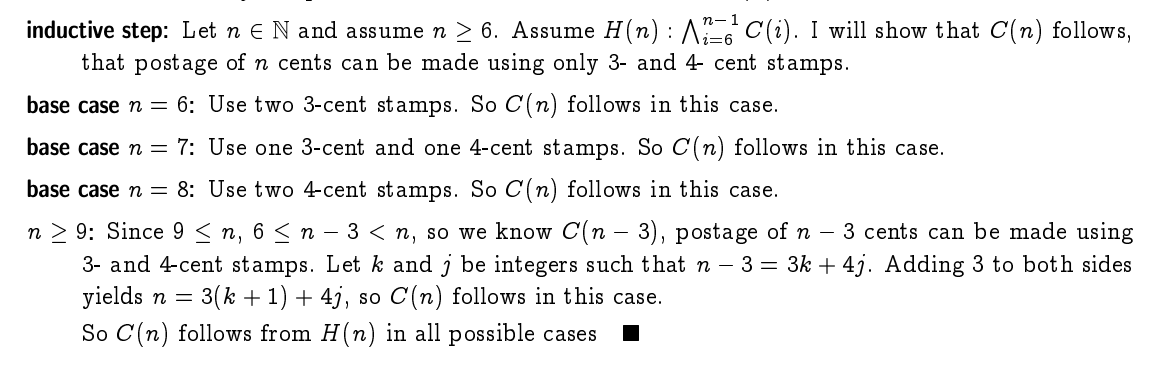
\includegraphics[width=\linewidth]{images/worksheet_2_question_2_note_1.png}
        \end{center}

        \item Noticed professor's note uses \textbf{thus} and \textbf{in other words} to
        unwrap statement further.

        \begin{mdframed}
        We will prove that $P(i + 1)$ holds, i.e., that we can make i + 1 cents
        of postage using only 4-cent and 7-cent stamps. In other words,
        we must prove that there are $k'$, $\ell' \in \mathbb{N}$ such that
        $4 \cdot k' + 7 \cdot \ell' = i + 1$.
        \end{mdframed}
    \end{itemize}

    % \bigskip

    % \begin{mdframed}
    %     \underline{\textbf{Rough Work:}}

    %     \bigskip

    %     Let $P(n)$ be the predicate defined as follows

    %     \bigskip

    %     \begin{center}
    %         $P(n)$: Postage of exactly $n$ cents can be made using only 3-cent and 4-cent stamps
    %     \end{center}

    %     \bigskip

    %     We will use complete induction to prove the statement holds for $n \geq 13$.

    %     \begin{enumerate}[1.]
    %         \item Base Case ($n = 13$)

    %         \begin{mdframed}
    %         \underline{\textbf{Base Case ($n = 13$):}}

    %         \bigskip

    %         Let $n = 13$.

    %         \bigskip

    %         We need to prove the statement is true for $n = 13$. That is, the
    %         postage of exactly 13 cents can be made using only 3-cent and 4-cent.

    %         \bigskip

    %         Because we know $(3 \cdot 3) + (1 \cdot 4)=13$, we can conclude the statement holds.

    %         \end{mdframed}

    %         \item Base Case ($n = 14$)

    %         \begin{mdframed}
    %         \underline{\textbf{Base Case ($n = 14$):}}

    %         \bigskip

    %         Let $n = 14$.

    %         \bigskip

    %         We need to prove the statement is true for $n = 14$. That is, the
    %         postage of exactly 14 cents can be made using only 3-cent and 4-cent.

    %         \bigskip

    %         Because we know $(2 \cdot 3) + (2 \cdot 4)=14$, we can conclude the statement holds.

    %         \end{mdframed}

    %         \item Base Case ($n = 15$)

    %         \begin{mdframed}
    %         \underline{\textbf{Base Case ($n = 15$):}}

    %         \bigskip

    %         Let $n = 15$.

    %         \bigskip

    %         We need to prove the statement is true for $n = 15$. That is, the
    %         postage of exactly 15 cents can be made using only 3-cent and 4-cent.

    %         \bigskip

    %         Because we know $(1 \cdot 3) + (3 \cdot 4)=15$, we can conclude the statement holds.

    %         \end{mdframed}

    %         \item Base Case ($n = 16$)

    %         \begin{mdframed}
    %         \underline{\textbf{Base Case ($n = 16$):}}

    %         \bigskip

    %         Let $n = 16$.

    %         \bigskip

    %         We need to prove the statement is true for $n = 16$. That is, the
    %         postage of exactly 16 cents can be made using only 3-cent and 4-cent.

    %         \bigskip

    %         Because we know $(4 \cdot 3) + (1 \cdot 4)=16$, we can conclude the statement holds.

    %         \end{mdframed}

    %         \item Base Case ($n = 17$)

    %         \begin{mdframed}
    %         \underline{\textbf{Base Case ($n = 17$):}}

    %         \bigskip

    %         Let $n = 17$.

    %         \bigskip

    %         We need to prove the statement is true for $n = 17$. That is, the
    %         postage of exactly 17 cents can be made using only 3-cent and 4-cent.

    %         \bigskip

    %         Because we know $(3 \cdot 3) + (2 \cdot 4)=17$, we can conclude the statement holds.

    %         \end{mdframed}

    %         \item Inductive Step

    %         \bigskip

    %         Let $i \in \mathbb{N}$ such that $i \geq 13$. Suppose that $P(i)$ holds. That is, the postage of
    %         exactly $i$ cents can be made using only 3-cent and 4-cent stamps. In other words,
    %         $\exists k, \ell \in \mathbb{N}$, $k \cdot 3 + \ell \cdot 4 = i$.

    %         \bigskip

    %         We need to prove the statement is true for $P(i+1)$. That is, the postage
    %         of exactly $i+1$ cents can be made using only 3-cent and 4-cent stamps. In other
    %         words, we need to prove $\exists k', \ell' \in \mathbb{N},\:
    %         3k' + 4\ell' = i + 1$. There are two cases: $\ell > 0$
    %         or $\ell = 0$.

    %         \bigskip

    %         We will use proof by cases.

    %         \begin{enumerate}[1.]
    %             \item Case 1 ($\ell > 0$):

    %             \bigskip

    %             Assume $\ell > 0$.

    %             \bigskip

    %             We need to prove $\exists k',\:\ell' \in \mathbb{N},\:3k' + 4\ell' = i + 1$.

    %             \bigskip

    %             Let $k' = k + 3$ and $\ell' = \ell - 2$ (where $\ell - 2$ is possible
    %             since $\ell > 0$).

    %             \begin{itemize}
    %                 \item Show $3k' + 4\ell' = 3 \cdot k + 4 \cdot l + 1$, starting from the left, using the facts

    %                 \begin{mdframed}
    %                 Starting from the left hand side, using the facts $k' = k + 3$ and $\ell' = \ell - 2$, we can write

    %                 \setcounter{equation}{0}
    %                 \begin{align}
    %                     3k' + 4\ell' &= (k+3) \cdot 3 + (\ell-2) \cdot 4\\
    %                     &= 3 \cdot k + 9 + 4 \cdot \ell - 8\\
    %                     &= 3 \cdot k + 4 \cdot \ell + 1\\
    %                     &= (3 \cdot k + 4 \cdot \ell) + 1
    %                 \end{align}

    %                 \end{mdframed}

    %                 \item Conclude $3k' + 4\ell' = i + 1$, using induction hypothesis.

    %                 \begin{mdframed}
    %                     Then, using induction hypothesis, i.e. $k \cdot 3 + \ell \cdot 4 = i$, we can conclude

    %                     \begin{align}
    %                         3k' + 4\ell' &= i + 1
    %                     \end{align}
    %                 \end{mdframed}
    %             \end{itemize}

    %             \bigskip

    %             \begin{mdframed}
    %             \underline{\textbf{Case 1 ($\ell > 0$):}}

    %             \bigskip

    %             Assume $\ell > 0$.

    %             \bigskip

    %             We need to prove $\exists k',\:\ell' \in \mathbb{N},\:3k' + 4\ell' = i + 1$.

    %             \bigskip

    %             Let $k' = k + 3$ and $\ell' = \ell - 2$ (where $\ell - 2$ is possible
    %             since $\ell > 0$).

    %             \bigskip

    %             Starting from the left hand side, using the facts $k' = k + 3$ and $\ell' = \ell - 2$, we can write

    %             \setcounter{equation}{0}
    %             \begin{align}
    %                 3k' + 4\ell' &= (k+3) \cdot 3 + (\ell-2) \cdot 4\\
    %                 &= 3 \cdot k + 9 + 4 \cdot \ell - 8\\
    %                 &= 3 \cdot k + 4 \cdot \ell + 1\\
    %                 &= (3 \cdot k + 4 \cdot \ell) + 1
    %             \end{align}

    %             \bigskip

    %             Then, using induction hypothesis, i.e. $k \cdot 3 + \ell \cdot 4 = i$, we can conclude

    %             \begin{align}
    %                 3k' + 4\ell' &= i + 1
    %             \end{align}
    %             \end{mdframed}

    %             \item Case 2 ($\ell = 0$):

    %             \bigskip

    %             Assume $\ell = 0$.

    %             \bigskip

    %             We need to prove $\exists k',\:\ell' \in \mathbb{N},\:3k' + 4\ell' = i + 1$.

    %             \bigskip

    %             \begin{itemize}
    %                 \item Find the value of $k'$.

    %                 \bigskip

    %                 First, we need to choose the value of $k'$.

    %                 \bigskip

    %                 \begin{itemize}
    %                     \item Show that $k \geq 6$ using the fact $\ell = 0$ and $3k + 4\ell = i$

    %                     \begin{mdframed}
    %                     The header tells us

    %                     \begin{align}
    %                         3 \cdot k + 4 \cdot \ell = i
    %                     \end{align}

    %                     \bigskip

    %                     Using the fact $\ell = 0$, we can write

    %                     \begin{align}
    %                         3 \cdot k &= i\\
    %                         k &= \frac{i}{3}
    %                     \end{align}

    %                     \bigskip

    %                     Then, because we know $i \geq 18$, we can write $k \geq 6$.
    %                     \end{mdframed}

    %                     \item Conclude by choosing $k' = k - 5$

    %                     \begin{mdframed}
    %                     Then, since $k'$ must be a natural number and $k \geq 6$, let $k' = k - 5$.
    %                     \end{mdframed}
    %                 \end{itemize}

    %                 \begin{mdframed}
    %                 First, we need to choose the value of $k'$.

    %                 \bigskip

    %                 The header tells us

    %                 \begin{align}
    %                     3 \cdot k + 4 \cdot \ell = i
    %                 \end{align}

    %                 \bigskip

    %                 Using the fact $\ell = 0$, we can write

    %                 \begin{align}
    %                     3 \cdot k &= i\\
    %                     k &= \frac{i}{3}
    %                 \end{align}

    %                 \bigskip

    %                 Then, because we know $i \geq 18$, we can write $k \geq 6$.

    %                 \bigskip

    %                 Then, since $k'$ must be a natural number and $k \geq 6$, let $k' = k - 5$.

    %                 \end{mdframed}

    %                 \item Find the value of $\ell'$

    %                 \bigskip

    %                 Second, we need to choose the value of $\ell'$.

    %                 \begin{mdframed}
    %                 Second, we need to choose the value of $\ell'$.

    %                 \bigskip

    %                 Since we know $\ell = 0$, and since we want the total to increase from $i$ by 1
    %                 in $3 \cdot k' + 4 \cdot \ell$, let $\ell' = 4$.
    %                 \end{mdframed}

    %                 \item Show $3k' + 4\ell' = i + 1$ using the value of $\ell' = 4$ and $k' = k - 5$.

    %                 \begin{mdframed}
    %                 Finally, starting from the left, using the facts $k' = k - 5$ and $\ell' = 4$, we can write

    %                 \begin{align}
    %                 3k' + 4\ell' &= (k-5) \cdot 3 + 4 \cdot 4\\
    %                 &= 3k - 15 + 16\\
    %                 &= 3k + 1
    %                 \end{align}

    %                 \bigskip

    %                 Then, by the fact $4\ell = \ell = 0$, we can write

    %                 \begin{align}
    %                 3k' + 4\ell' &= 3k + 4\ell + 1\\
    %                 &= (3k + 4\ell) + 1
    %                 \end{align}

    %                 \bigskip

    %                 Then, by using inductive hypothesis, $3k + 4\ell = i$, we can conclude

    %                 \begin{align}
    %                 3k' + 4\ell' &= i + 1
    %                 \end{align}

    %                 \end{mdframed}
    %             \end{itemize}

    %             \bigskip

    %             \begin{mdframed}
    %             \underline{\textbf{Case 2 ($\ell = 0$):}}

    %             \bigskip

    %             First, we need to choose the value of $k'$.

    %             \bigskip

    %             The header tells us

    %             \begin{align}
    %                 3 \cdot k + 4 \cdot \ell = i
    %             \end{align}

    %             \bigskip

    %             Using the fact $\ell = 0$, we can write

    %             \begin{align}
    %                 3 \cdot k &= i\\
    %                 k &= \frac{i}{3}
    %             \end{align}

    %             \bigskip

    %             Then, because we know $i \geq 18$, we can write $k \geq 6$.

    %             \bigskip

    %             Then, since $k'$ must be a natural number and $k \geq 6$, let $k' = k - 5$.

    %             \bigskip

    %             Second, we need to choose the value of $\ell'$.

    %             \bigskip

    %             Since we know $\ell = 0$, and since we want the total to increase from $i$ by 1
    %             in $3 \cdot k' + 4 \cdot \ell$, let $\ell' = 4$.

    %             \bigskip

    %             Finally, starting from the left, using the facts $k' = k - 5$ and $\ell' = 4$, we can write

    %             \begin{align}
    %             3k' + 4\ell' &= (k-5) \cdot 3 + 4 \cdot 4\\
    %             &= 3k - 15 + 16\\
    %             &= 3k + 1
    %             \end{align}

    %             \bigskip

    %             Then, by the fact $4\ell = \ell = 0$, we can write

    %             \begin{align}
    %             3k' + 4\ell' &= 3k + 4\ell + 1\\
    %             &= (3k + 4\ell) + 1
    %             \end{align}

    %             \bigskip

    %             Then, by using inductive hypothesis, $3k + 4\ell = i$, we can conclude

    %             \begin{align}
    %             3k' + 4\ell' &= i + 1
    %             \end{align}

    %             \end{mdframed}
    %         \end{enumerate}
    %     \end{enumerate}
    % \end{mdframed}
\end{itemize}

\section*{Question 3}
\begin{itemize}
    \item

    \begin{mdframed}
        \underline{\textbf{Rough Work:}}

        \bigskip

        Define $C(n):$ $f(n) \leq 3^n$.

        \bigskip

        We will prove by complete induction that $\forall n \in \mathbb{N}, n \geq 2 \Rightarrow C(n)$.

        \bigskip

        \begin{itemize}
            \item Inductive Step

            \begin{mdframed}
            Let $n \in \mathbb{N}$ and assume $n \geq 2$. Assume $H(n):\:\bigwedge\limits_{i=0}^{n-1} C(i)$.

            \bigskip

            We need to prove $C(n)$ follows. That is, $f(n) \leq 3^n$.
            \end{mdframed}

            \item Base Case ($n = 0$)

            \begin{mdframed}
            \underline{\textbf{Base Case ($n = 0$):}}

            \bigskip

            Let $n = 0$.

            \bigskip

            We need to prove $C(0)$ is true. That is, $f(0) \leq 3^0$.

            \bigskip

            The definition of $f(n)$ tells us that $f(0) = 1$.

            \bigskip

            Using this fact, we can conclude

            \begin{align}
                f(0) = 1 &\leq 1\\
                &\leq 3^0
            \end{align}
            \end{mdframed}

            \item Base Case ($n = 1$)

            Let $n = 1$.

            \bigskip

            We need to prove $C(1)$ is true. That is, $f(1) \leq 3^1$.

            \begin{mdframed}

            \underline{\textbf{Base Case ($n = 1$):}}

            \bigskip

            Let $n = 1$.

            \bigskip

            We need to prove $C(1)$ is true. That is, $f(1) \leq 3$.

            \bigskip

            The definition of $f(n)$ tells us that $f(1) = 3$.

            \bigskip

            Using this fact, we can conclude

            \begin{align}
                f(1) = 3 &\leq 3\\
                &\leq 3^1
            \end{align}

            \end{mdframed}

            \item $n \geq 2$
        \end{itemize}
    \end{mdframed}
\end{itemize}

\end{document}